
\chapter{Estado da Arte}
\label{chapter:stateofart}

\begin{introduction}
Este capítulo revê as soluções existentes de mesas sísmicas, tanto comerciais como académicas de baixo custo, e identifica as lacunas que motivaram o presente projeto.
\end{introduction}

\section{Mesas Sísmicas --- Conceito e Aplicações}
\label{sec:conceito}

Uma mesa sísmica é um equipamento que reproduz movimentos causados por sismos para estudar a resposta dinâmica de estruturas e materiais em condições controladas. O princípio de funcionamento é direto: insere-se na plataforma um perfil de deslocamento, velocidade ou aceleração correspondente a um registo sísmico real ou sintético.

Do ponto de vista da configuração mecânica, as mesas sísmicas classificam-se principalmente em uni-axiais, bi-axiais e sistemas de seis graus de liberdade (6-DOF). Os sistemas uni-axiais simulam apenas uma componente horizontal do movimento; os bi-axiais reproduzem em simultâneo as componentes Norte-Sul e Este-Oeste de um registo sísmico, representando com maior fidelidade a realidade física de um evento~\cite{2DOF2025}.

\section{Soluções Comerciais Existentes}
\label{sec:comerciais}

No mercado académico e de investigação, a Quanser Inc. é o fabricante de referência para mesas sísmicas de bancada. A \textbf{Quanser Shake Table II XY}~\cite{QuanserShakeTableIIXY} é a solução bi-axial de entrada de gama desta empresa, constituída por dois módulos uni-axiais montados perpendicularmente. Cada eixo tem uma gama de deslocamento de $\pm7{,}6$~cm e o sistema atinge uma aceleração de 2,5~g com uma carga de 7,5~kg. O acionamento é feito por motores \textit{brushless} de corrente contínua de alta potência, com encoders de alta resolução (resolução linear de 1,55~\textmu m), e a plataforma suporta perfis de sismos reais pré-carregados (Northridge, Kobe, El~Centro) bem como registos personalizados obtidos da base de dados PEER. O controlo é efetuado via MATLAB\textsuperscript{\textregistered}/Simulink\textsuperscript{\textregistered} com o software QUARC\textsuperscript{\textregistered} da Quanser.

% TODO: Inserir figura da Quanser Shake Table II XY para ilustrar a solução comercial de referência.
\begin{figure}[H]
 \centering
 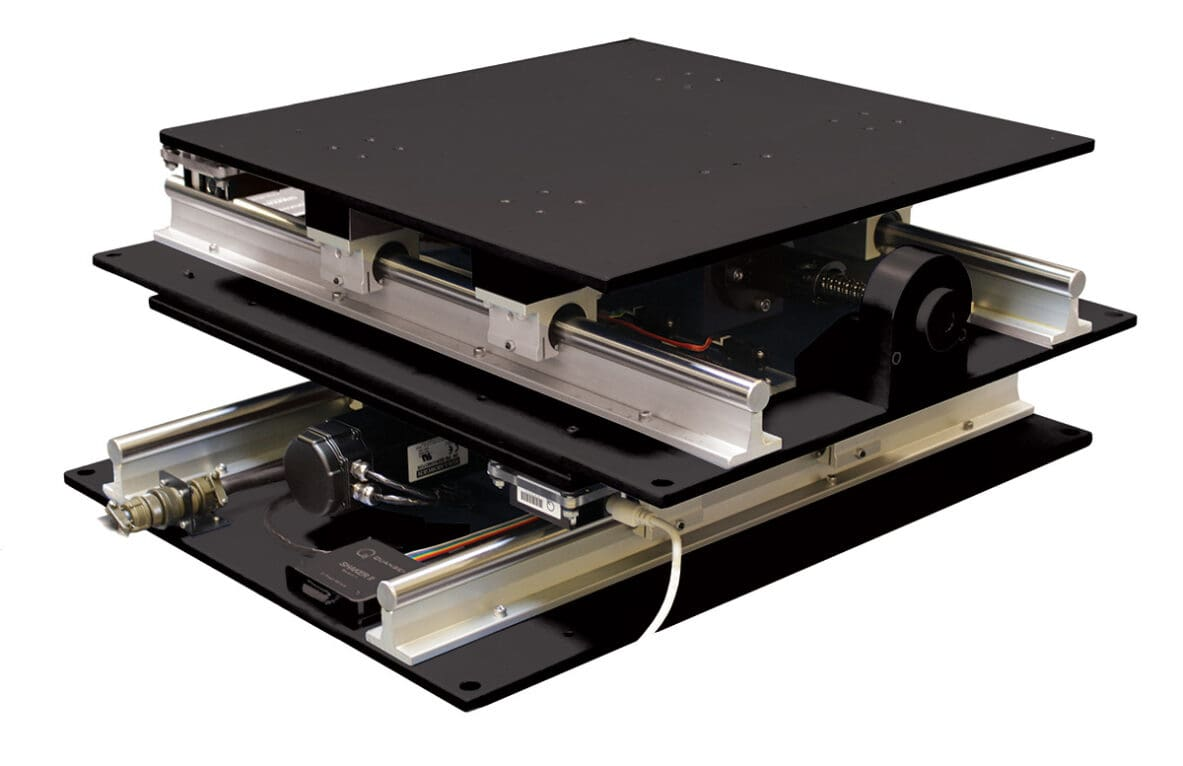
\includegraphics[width=0.6\textwidth]{figs/quanser_shake_table.jpg}
 \caption{Quanser Shake Table II XY --- solução comercial bi-axial de referência. Fonte:~\cite{QuanserShakeTableIIXY}.}
 \label{fig:quanser}
\end{figure}

Para necessidades de maior capacidade de carga, a \textbf{Quanser Shake Table III XY}~\cite{QuanserShakeTableIII} oferece uma plataforma bi-axial acionada por motores lineares, capaz de movimentar cargas até 100~kg com uma aceleração máxima de 1~g em cada eixo e uma gama de deslocamento de $\pm10{,}8$~cm.

\section{Projetos Académicos e Low-Cost}
\label{sec:academicos}

A dificuldade de acesso a equipamento comercial motivou, ao longo das últimas décadas, o desenvolvimento de diversas alternativas académicas de baixo custo.

O trabalho de Damcı e Şekerci~\cite{Damci2018} é uma das referências mais citadas nesta área. Os autores desenvolveram a mesa sísmica \textbf{SARSAR}, uma plataforma uni-axial de baixo custo baseada em microcontroladores Arduino. O sistema utiliza um fuso de esferas acionado por um motor de passo para transferir registos de aceleração de sismos reais ao longo de um único eixo horizontal. Para verificação, a resposta da mesa é medida por uma unidade de aquisição de dados independente baseada num Arduino MEGA. A plataforma consegue deslocamentos até $\pm75$~mm, velocidades até 350~mm/s e frequências até 17~Hz.

% TODO: Inserir foto ou imagem do protótipo SARSAR.
\begin{figure}[h]
 \centering
 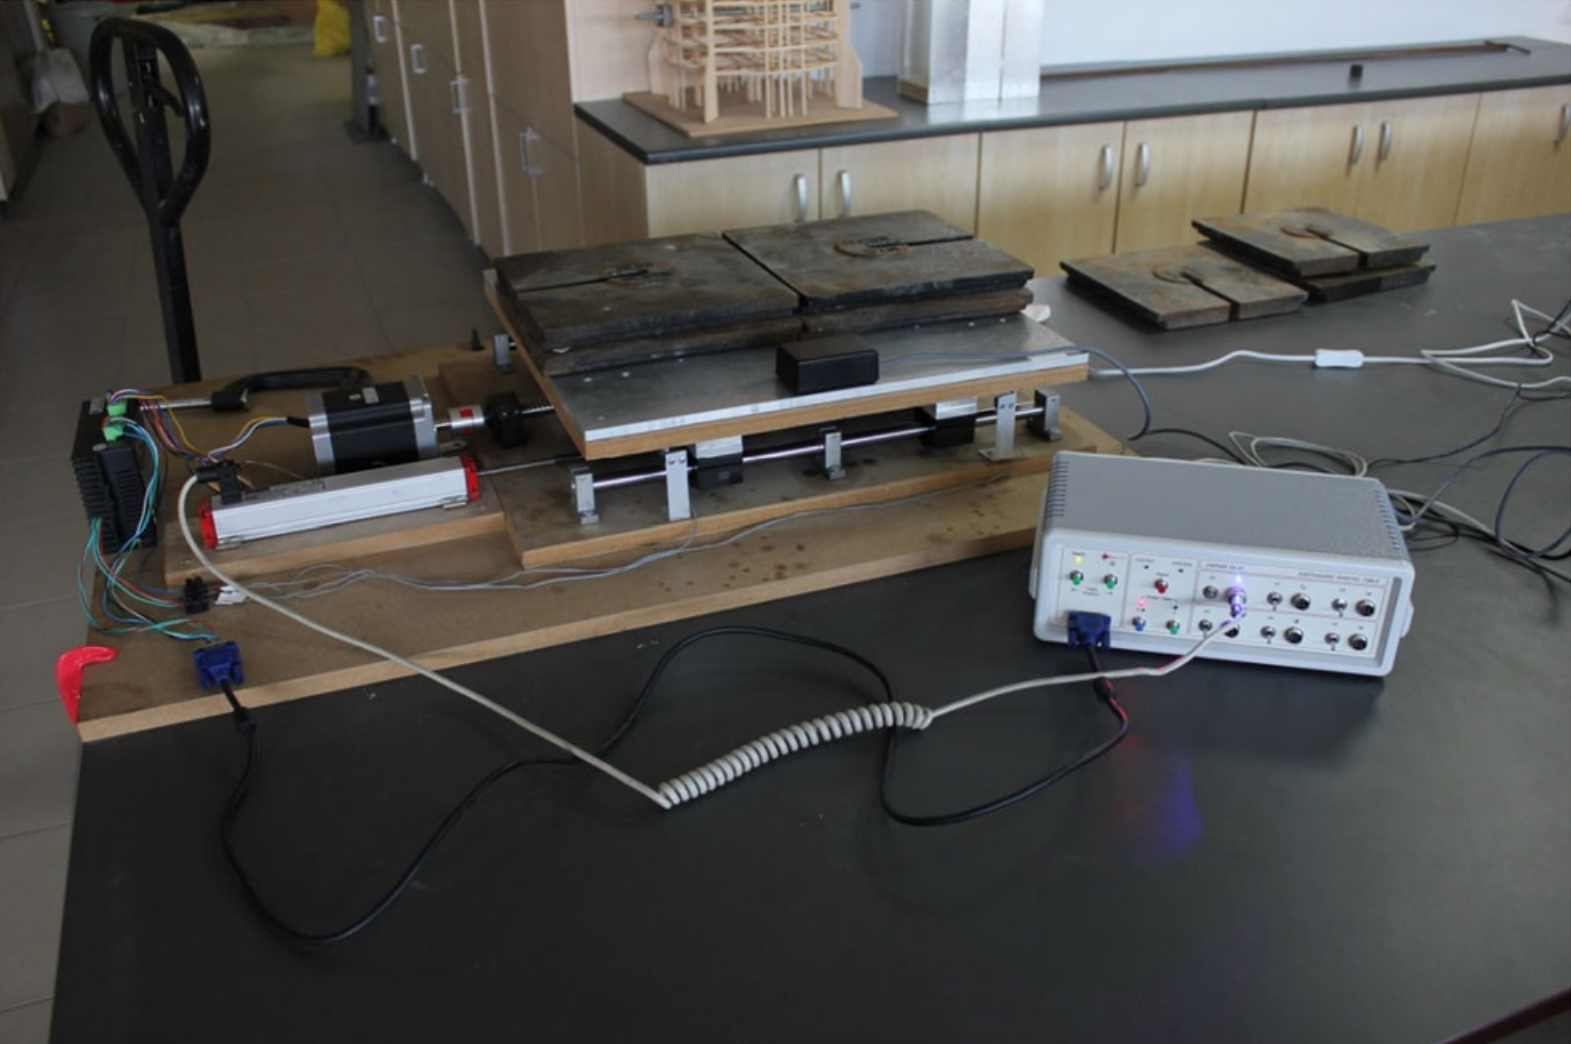
\includegraphics[width=0.55\textwidth]{figs/sarsar.png}
 \caption{Mesa sísmica SARSAR, baseada em Arduino, desenvolvida por Damcı e Şekerci~\cite{Damci2018}.}
 \label{fig:sarsar}
\end{figure}

Mais recentemente, Chen et al.~\cite{Shakebot2022} apresentaram o \textbf{Shakebot}, uma mesa sísmica uni-axial \textit{open-source} com um custo inferior a 2\,000~USD, construída com base no sistema operativo robótico ROS (\textit{Robot Operating System}). Uma característica distintiva é a reutilização de componentes de impressoras 3D de alta precisão, nomeadamente um motor de passo em malha fechada para o acionamento e uma correia dentada para a transmissão. O sistema atinge uma aceleração máxima de 11,8~m/s² (1,2~g) e uma velocidade de 0,5~m/s com uma carga de 2~kg, com acelerómetro e câmara de alta cadência integrados para estimação do movimento da plataforma.

% TODO: Inserir foto ou imagem do Shakebot.
\begin{figure}[h]
 \centering
 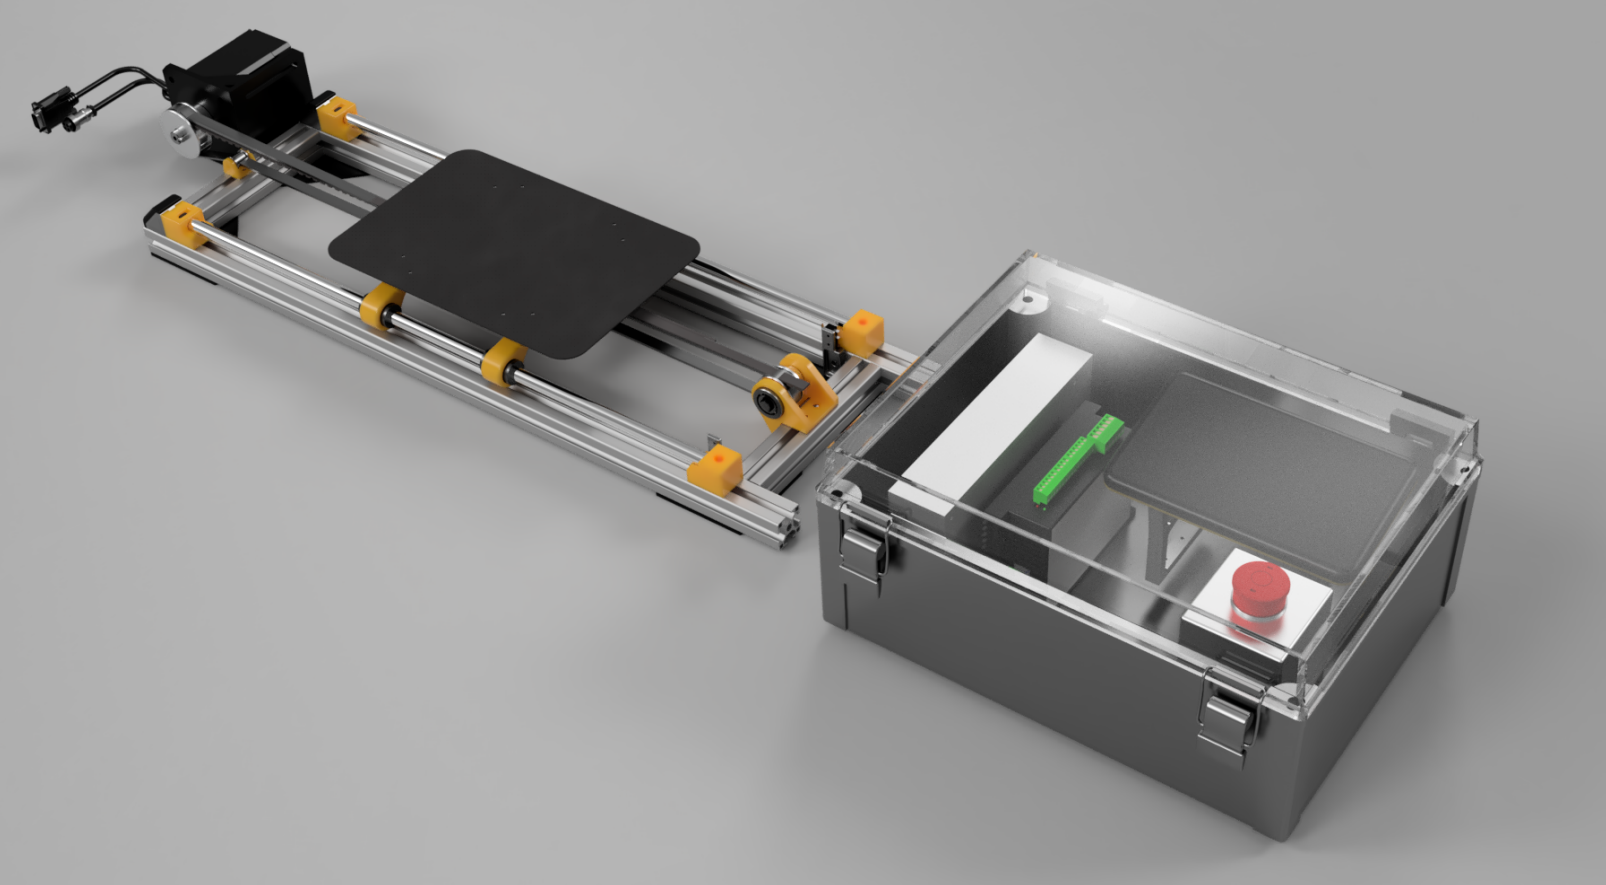
\includegraphics[width=0.55\textwidth]{figs/shakebot.png}
 \caption{Mesa sísmica Shakebot (CAD), open-source baseada em ROS~\cite{Shakebot2022}.}
 \label{fig:shakebot}
\end{figure}

Vargas et al.~\cite{2DOF2025} apresentam um projeto de maior ambição: o desenvolvimento de uma mesa de \textbf{2-DOF de arquitetura aberta}, capaz de reproduzir registos sísmicos reais em dois eixos horizontais ortogonais. A plataforma é construída com módulos CNC standard e motores NEMA23 sem escovas (\textit{BLDC}), com uma estrutura base em aço estrutural de alta inércia para minimizar vibrações parasitas. O contributo mais relevante deste trabalho é a caracterização das dinâmicas não lineares de atrito do sistema (nomeadamente os efeitos de amortecimento viscoso e de Coulomb), recorrendo ao algoritmo de Mínimos Quadrados Recursivos (RLS) com filtros de variável de estado (SVF) para identificação de parâmetros. Esta modelação é indispensável para a reprodução fiel de cruzamentos de velocidade zero nos sinais sísmicos.

% TODO: Inserir foto ou imagem da mesa 2-DOF.
\begin{figure}[h]
 \centering
 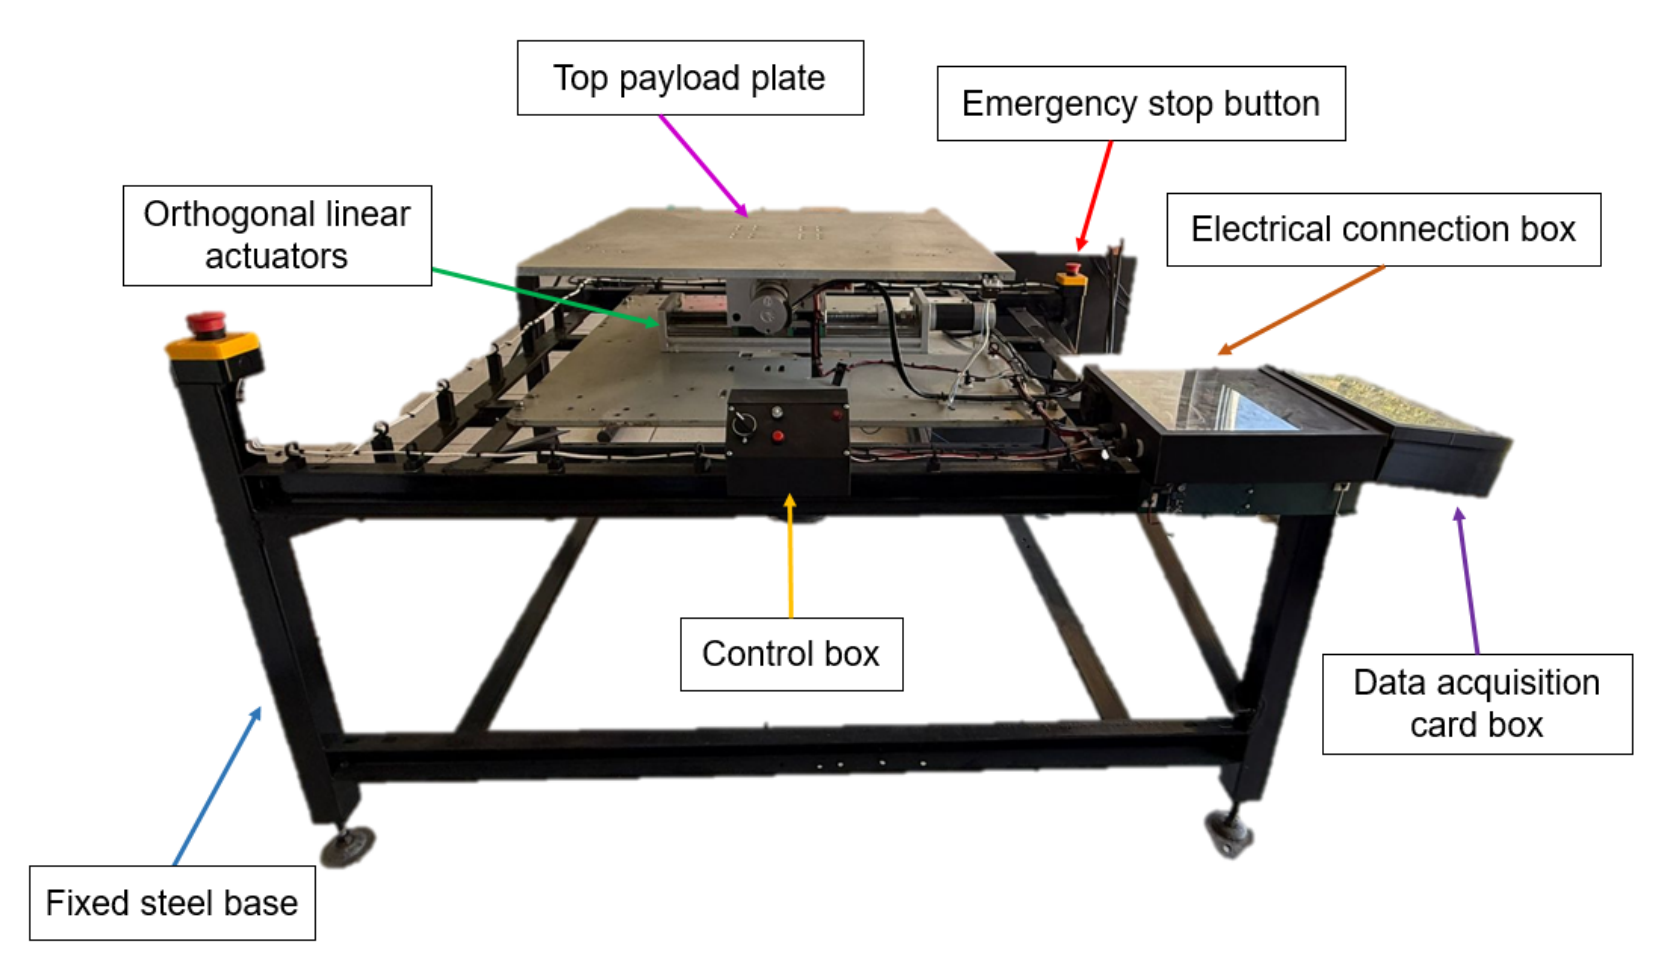
\includegraphics[width=0.55\textwidth]{figs/mesa2dof.png}
 \caption{Mesa sísmica 2-DOF de arquitetura aberta~\cite{2DOF2025}.}
 \label{fig:mesa2dof}
\end{figure}

\section{Análise Comparativa e Lacunas Identificadas}
\label{sec:comparativo}

A Tabela~\ref{tab:comparativo} sintetiza as principais características dos sistemas analisados, confrontando-os com o projeto desenvolvido no presente trabalho.

\begin{table}[h]
\centering
\caption{Comparação entre soluções de mesas sísmicas existentes e o presente projeto.}
\label{tab:comparativo}
\begin{tabular}{lccc}
\hline
\textbf{Solução} & \textbf{Eixos} & \textbf{Custo} & \textbf{Imp. 3D} \\
\hline
Quanser Shake Table II XY~\cite{QuanserShakeTableIIXY} & 2 & $>$10\,000~€ & Não \\
Quanser Shake Table III XY~\cite{QuanserShakeTableIII} & 2 & $>>$10\,000~€ & Não \\
SARSAR~\cite{Damci2018}                                & 1 & 770~USD & Não \\
Shakebot~\cite{Shakebot2022}                           & 1 & 1\,300~USD & Parcial \\
Mesa 2-DOF~\cite{2DOF2025}                             & 2 & 1\,500~USD* & Não \\
\textbf{Este projeto}                                  & \textbf{2} & \textbf{$<$500~€} & \textbf{Sim} \\
\hline
\multicolumn{3}{l}{%
  \footnotesize * O custo reportado (1\,500~USD) não contabiliza um componente já existente em laboratório,}\\
\multicolumn{3}{l}{%
  \footnotesize \phantom{* }avaliado em 1\,000~USD. O custo total real estimado da mesa é de 2\,500~USD.}\\
\end{tabular}
\end{table}

Da análise comparativa ressaltam duas conclusões principais. As soluções comerciais bi-axiais disponíveis, nomeadamente as da Quanser, têm um custo proibitivo para utilização em contextos de recursos limitados e dependem de ecossistemas de software proprietários. Os projetos académicos de baixo custo existentes são, na sua maioria, uni-axiais.

O único projeto bi-axial de arquitetura aberta identificado na literatura~\cite{2DOF2025} utiliza materiais e componentes industriais que aumentam significativamente o custo e a complexidade de fabrico, não sendo adequado para utilização portátil em trabalho de campo.

Identificou-se assim uma lacuna clara: não existe, na literatura acessível, uma solução que combine simultaneamente dois eixos de atuação, com custo inferior a 500~€, arquitetura totalmente aberta e reproduzível. O presente projeto posiciona-se nessa interseção.
